\section{Introduktion}
%%%%%%%%%%%% MID WAY AGENDA %%%%%%%%%%%%%%
 \begin{frame}<beamer>
 \frametitle{Nicolaj Vinkel Christensen}
 \tableofcontents[currentsection]
 \end{frame}
% \AtBeginSection[] {
%     \begin{frame}<beamer>
%     \frametitle{Nicolaj Vinkel Christensen} %
%     \tableofcontents[currentsection]  
%     \end{frame}
%     \lattersubsectfalse
% }
%%%%%%%%%%%% MID WAY AGENDA %%%%%%%%%%%%%%

\subsection*{Optimering af containerkraner}
\begin{frame}{Introduktion}{Optimering af containerkraner}


 \begin{minipage}[t]{0.45\linewidth}
  \begin{itemize}
    \item<1-> Effektivitet af containerkraner 
        \begin{itemize}
          \item<1-> Der bliver fragtet 651 mio. container om året.
          \item<1-> Mere effektive kraner leder til mere overskud. 
        \end{itemize}
  \end{itemize}
  \end{minipage}
  \begin{minipage}[t]{0.42\linewidth}
    \begin{itemize}
      \item<1->[] {
\scalebox{0.8}{
 \centering
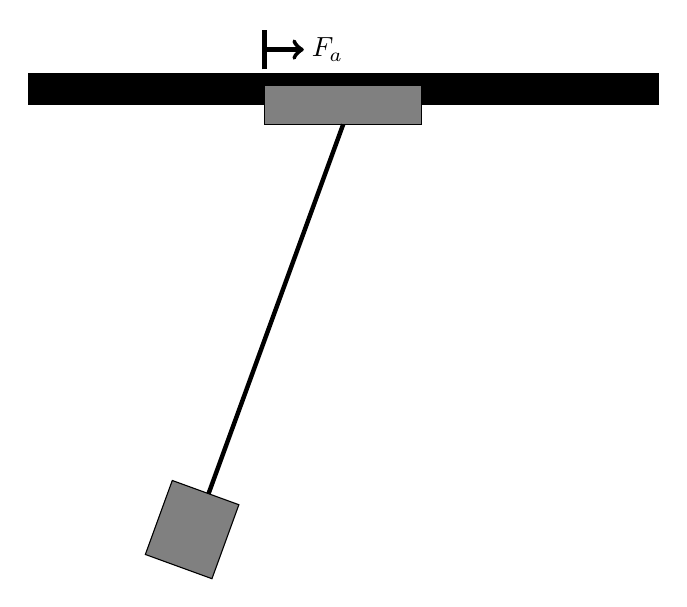
\begin{tikzpicture}
	\draw [ultra thick] (-1,0.7) -- (-1,1.2);
	\draw [->,ultra thick] (-1,0.95) -- (-0.5,0.95);
	\node at (-0.2,0.95) {$F_a$};
	%\node at (-2.32,-6.38) {$\Delta \theta$};
	

	\draw [fill = black] (-4,0.25) rectangle (4,0.65);
	\draw [fill = gray] (-1,0) rectangle (1,0.5);

	%\draw [dashed] (0,-0) -- (-1.07,-6.1); % 260
	\draw [ultra thick] (0,0) -- (-1.71,-4.69);  % 250
	%\draw [dashed] (0,0) -- (-3.1,-5.36);   % 240

	%\draw [<->,dashed] (-1.1,-6.17) arc [radius=6.2, start angle=260, end angle= 240];

	\draw[fill = gray,rotate around={-20:(-1.71,-4.69)}] (-2.2,-4.69) rectangle (-1.3,-5.69);
\end{tikzpicture}}}
    \end{itemize}                   
  \end{minipage}
  \end{frame}


%%%%%%%%%%%%%%%%%%%%%%%%%%%%%%%%%%%%%%%%%%% 

\begin{frame}{Introduktion}{Optimering af containerkraner}


 \begin{minipage}[t]{0.45\linewidth}
  \begin{itemize}
    \item<1-> Effektivitet af containerkraner 
        \begin{itemize}
          \item<1-> Der bliver fragtet 651 mio. container om året.
          \item<1-> Mere effektive kraner leder til mere overskud. 
        \end{itemize}
    \item<1-> Problemformulering
        \begin{itemize}
          \item<1-> \textit{"How can a control system be designed to automatically operate a crane."}
        \end{itemize}
  \end{itemize}
  \end{minipage}
  \begin{minipage}[t]{0.42\linewidth}
    \begin{itemize}
      \item<1->[] {
\scalebox{0.8}{
 \centering
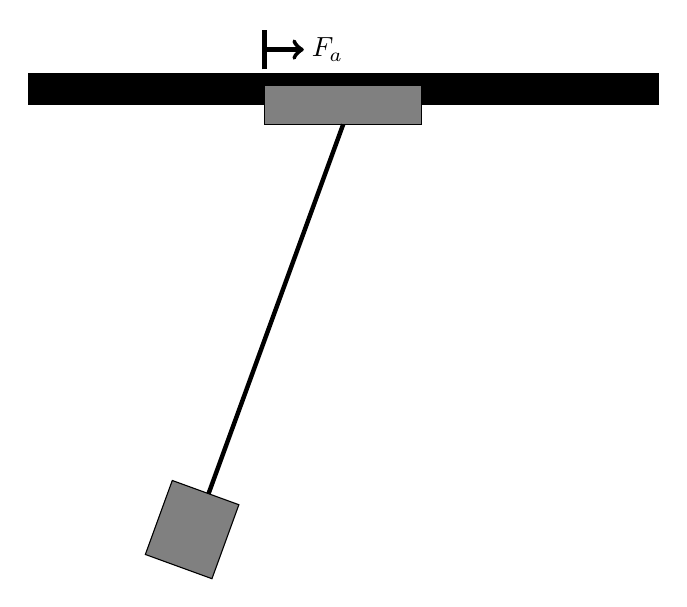
\begin{tikzpicture}
	\draw [ultra thick] (-1,0.7) -- (-1,1.2);
	\draw [->,ultra thick] (-1,0.95) -- (-0.5,0.95);
	\node at (-0.2,0.95) {$F_a$};
%	\node at (-2.32,-6.38) {$\Delta \theta$};
	

	\draw [fill = black] (-4,0.25) rectangle (4,0.65);
	\draw [fill = gray] (-1,0) rectangle (1,0.5);

%	\draw [dashed] (0,-0) -- (-1.07,-6.1); % 260
	\draw [ultra thick] (0,0) -- (-1.71,-4.69);  % 250%
%	\draw [dashed] (0,0) -- (-3.1,-5.36);   % 240

%	\draw [<->,dashed] (-1.1,-6.17) arc [radius=6.2, start angle=260, end angle= 240];

	\draw[fill = gray,rotate around={-20:(-1.71,-4.69)}] (-2.2,-4.69) rectangle (-1.3,-5.69);
\end{tikzpicture}}}
    \end{itemize}                   
  \end{minipage}
  \end{frame}


%%%%%%%%%%%%%%%%%%%%%%%%%%%%%%%%%%%%%%%%%%%%% 
\section{Opbygning af kran}
 \begin{frame}<beamer>
 \frametitle{Nicolaj Vinkel Christensen}
 \tableofcontents[currentsection]
 \end{frame}
\begin{frame}{Opbygning af kran}{Eksisterende setup}


 \begin{minipage}[H]{0.8\linewidth}
  \begin{itemize}
    \item<1-> Udgangspunkt i model kran 
        \begin{itemize}
          \item<1-> Eksisterende setup
              \begin{itemize}
              \item<1-> Trolley, elektromagnet, motor og gearing. 
              \item<1-> Sensore, effektforstærker forsyning. 
              \end{itemize}
        \end{itemize}
  \end{itemize}
  \end{minipage}
  \begin{minipage}[H]{0.6\linewidth}
    \begin{itemize}
      \item<1->[] {
              %\begin{figure}[H]
              %\centering
              %\end{figure}
              }
    \end{itemize}                   
  \end{minipage}
    \begin{center}
              \includegraphics[width=0.8\textwidth]{Billeder/FullCrane}
    \end{center}
 \end{frame}

%%%%%%%%%%%%%%%%%%%%%%%%%%%%%%%%%%%%%%%%%%%%% 

\begin{frame}{Opbygning af kran}{Forbedringer af kranen}


 \begin{minipage}[H]{0.3\linewidth}
  \begin{itemize}
    \item<1-> Forbedringer 
    \vspace{0.2cm}
        \begin{itemize}
          \item<1-> Kontrol platform
          \vspace{0.2cm}
          \item<1-> Forsyning 
        \end{itemize}
  \end{itemize}
  \end{minipage}

  \vfill
  \begin{center}
  \begin{tikzpicture}

%Boxes
\node[fill = white,box] (Sensor) at (0,0) {Sensor};
\node[fill = white,box] (Con) at ($(3,0)+(Sensor)$) {Kontrol \\ platform};
\node[fill = white,box] (driv) at ($(3,0)+(Con)$) {Forsyning};
\node[fill = white,box] (Mot) at ($(3,0)+(driv)$) {DC \\ Motor};
%connections
\draw[->, ultra thick] (Sensor) -- (Con);
\draw[->, ultra thick] (Con) -- (driv);
\draw[->, ultra thick] (driv) -- (Mot);
\end{tikzpicture}%
\end{center}
  \end{frame}


  %%%%%%%%%%%%%%%%%%%%%%%%%%%%%%%%%%%%%%%%%%%%%%%%%%%%%

\begin{frame}{Opbygning af kran}{Forbedringer af kranen}


 \begin{minipage}[H]{0.3\linewidth}
  \begin{itemize}
    \item<1-> Forbedringer 
        \begin{itemize}
          \item<1-> Kontrol platform
            \begin{itemize}
              \item<1-> FPGA
              \item<1-> ADC
            \end{itemize}
          \item<1-> Forsyning 
            \begin{itemize}
              \item<1-> Motor drivere 
            \end{itemize}
          \item<1-> Fjernbetjening 
        \end{itemize}
  \end{itemize}
\end{minipage}

  \vfill

  \begin{center}
  \scalebox{0.8}{
  \begin{tikzpicture}
%Boxes
\node[fill = white,box] (Sensor) at (0,0) {Sensor};
\node[fill = white,box] (ADC) at ($(3,0)+(Sensor)$) {ADC};
\node[fill = white,box] (Con) at ($(3,0)+(ADC)$) {FPGA};
\node[fill = white,box] (driv) at ($(3,0)+(Con)$) {Motor \\ driver};
\node[fill = white,box] (Mot) at ($(3,0)+(driv)$) {DC \\ Motor};
\node[fill = white,box] (RC) at ($(0,-2)+(Sensor)$) {Remote \\ Control};
%connections
\draw[->, ultra thick] (Sensor) -- (ADC);
\draw[->, ultra thick] (ADC) -- (Con);
\draw[->, ultra thick] (Con) -- (driv);
\draw[->, ultra thick] (driv) -- (Mot);
\draw[->, ultra thick] ([yshift=0.3cm]RC.east) -| (ADC);
\draw[->, ultra thick] ([yshift=-0.3cm]RC.east) -| (Con);
\end{tikzpicture}}
\end{center}
  \end{frame}


  %%%%%%%%%%%%%%%%%%%%%%%%%%%%%%%%%%%%%%%%%%%%%%%%%%%%%

\begin{frame}{Opbygning af kran}{Forbedringer af kranen}

\begin{columns}[T]
\begin{column}{.35\textwidth}

  \begin{itemize}
    \item<1-> FPGA
        \begin{itemize}
          \item<1-> Papilio Duo
        \end{itemize}
    \vspace{0.8cm}
    \item<2-> Motor drivere
        \begin{itemize}
          \item<1-> Escon 50/5  
        \end{itemize}
    \vspace{0.8cm}
    \item<3-> ADC
        \begin{itemize}
          \item<1-> Papilio Analog Wing 
        \end{itemize}
  \end{itemize}
\end{column}%
\hfill%
\begin{column}{.65\textwidth}

\vspace{-0.7cm}
\begin{figure}[H]
  \centering
\onslide<1->  \begin{subfigure}{0.98\textwidth}
        \centering
        \includegraphics[width=0.5\textwidth]{Billeder/Papilio_DUO}
        \end{subfigure}
\onslide<2->  \begin{subfigure}{0.98\textwidth}
        \centering
        \includegraphics[width=0.5\textwidth]{Billeder/Escon_fig}
        \end{subfigure}
\onslide<3->  \begin{subfigure}{0.98\textwidth}
        \centering
        \includegraphics[width=0.5\textwidth]{Billeder/Analog_wing}
        \end{subfigure}     
\end{figure}

\end{column}
\end{columns}

  \end{frame}



%%%%%%%%%%%%%%%%%%%%%%%%%%%%%%%%%%%%%%% 
\section{Krav}
 \begin{frame}<beamer>
 \frametitle{Nicolaj Vinkel Christensen}
 \tableofcontents[currentsection]
 \end{frame}
\begin{frame}{Krav}{Hvordan skal kranen bevæge sig?}


 \begin{minipage}[H]{0.8\linewidth}
  \begin{itemize}
    \item<1-> Metoder: 
    \vspace{0.2cm}
        \begin{itemize}
          \item<1-> \textbf{(1)} Bevægelse i x- og y-aksen samtidig.
          \vspace{0.2cm}
          \item<1-> \textbf{(2)} Bevægelse i x- og y-aksen sekventielt.
        \end{itemize}
  \end{itemize}
  \end{minipage}

  \vfill
\begin{center}
\begin{figure}[H]
  \centering
  \begin{subfigure}[b]{.48\textwidth}
    \centering
      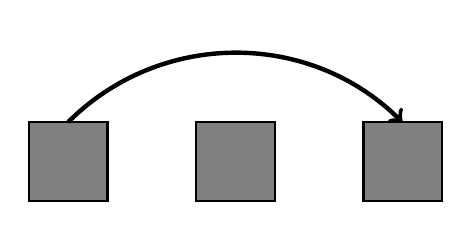
\begin{tikzpicture}
      \draw [fill=gray, thick](0,0) rectangle (1,1);
      \draw [fill=gray, thick](4.25,0) rectangle (5.25,1);
      \draw [fill=gray, thick](2.125,0) rectangle (3.125,1);

      \draw [->, ultra thick] (0.5,1) arc [radius=3, start angle=135, end angle= 45];
      \end{tikzpicture}
      \caption*{Metode \textbf{(1)}}
%    \hspace{-6cm}
  \end{subfigure}
  \begin{subfigure}[b]{.48\textwidth}
    \centering
        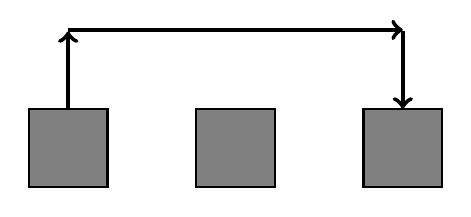
\begin{tikzpicture}
        \draw [fill=gray, thick](0,0) rectangle (1,1);
        \draw [fill=gray, thick](4.25,0) rectangle (5.25,1);
        \draw [fill=gray, thick](2.125,0) rectangle (3.125,1);

        \draw [->,ultra thick] (0.5,1) -- (0.5,1.98);
        \draw [->,ultra thick] (0.5,2) -- (4.75,2);
        \draw [->,ultra thick] (4.75,1.98) -- (4.75,1);
        \end{tikzpicture}
      \caption*{Metode \textbf{(2)}}
%    \hspace{6cm}
  \end{subfigure}
\end{figure}
\end{center}
  \end{frame}

%%%%%%%%%%%%%%%%%%%%%%%%%%%%%%%%%%%%%%% 
\begin{frame}{Krav}{Kravspecifikation}


 \begin{minipage}[H]{0.8\linewidth}
  \begin{itemize}
    \item<1-> Krav til de dynamiske egenskaber for kranen.
    \vspace{0.2cm}
        \begin{itemize}
          \item<1-> Opsat for positionen af elektromagneten. 
          \vspace{0.2cm}
          \item<1-> Opsat for x- og y-aksen individuelt.
        \end{itemize}
  \end{itemize}
  \end{minipage}
  \vfill
\begin{description}
    \item[\textbf{(A)}] : y-akse settling time for positiv retning , $t_s \leq 6,75 s$
    \item[\textbf{(B)}] : y-akse settling time for negativ retning, $t_s \leq 5,58 s$
    \item[\textbf{(C)}] : y-akse steady-state-error, $e_{ss} = 0,0\%$
    \item[\textbf{(D)}] : y-akse overshoot, $M_p = 0,0\%$ 
    \item[\textbf{(E)}] : x-akse settling time, $t_s \leq 17,45 s$
    \item[\textbf{(F)}] : x-akse steady-state-error, $e_{ss} = 0,0\%$ 
    \item[\textbf{(G)}] : x-akse overshoot, $M_p \leq 6,4\%$
\end{description}

  \end{frame}
